\documentclass[11pt]{article}
\usepackage[utf8]{inputenc}
\usepackage[T1]{fontenc}
\usepackage{graphicx}
\usepackage{booktabs}
\usepackage{amsmath}
\usepackage{amssymb}
\usepackage{hyperref}
\setlength{\emergencystretch}{2.5em}
\usepackage{geometry}
\geometry{a4paper, margin=2.4cm}
\usepackage{natbib}
\usepackage{enumitem}
\setlist{nosep}

\newcommand{\E}{\mathbb{E}}
\newcommand{\Prob}{\mathbb{P}}
\newcommand{\ind}{\mathbf{1}}

\title{\vspace{-1.2em}CrystalRL --- Crystal Clear Reinforcement Learning\\
\large Publication proposal: what does an agent gain when interpretability\\
is built in rather than explained after the fact?}
\author{Ivan Pavliuk}
\date{July 2026}

\begin{document}
\maketitle
\vspace{-2em}

\begin{abstract}
\noindent The field that studies how to explain reinforcement-learning (RL) agents has, by its
own account, a measurement problem: interpretability is routinely claimed and rarely measured,
and the surveys say so explicitly. We completed a study designed so the claim \emph{could
lose}. One trading agent was built three times: first as a strong conventional agent whose
decisions come from an unreadable learned state (a ``black box''); then the black box was kept
and the best available \emph{after-the-fact} explanation program was run over it; finally the
agent was rebuilt so that its entire memory is one \emph{named} number --- the probability
that the market is in a falling regime --- and its policy is a rule readable as a sentence.
All were scored with one number --- generations 1 and 2 share a score, because the
after-the-fact reading is the black box's only route to a human-sized story --- CrystalScore, which multiplies three measurable
properties: whether setting the agent's named internal belief to a chosen value changes its behavior
exactly as the name promises (faithfulness), whether a nine-rule
story can reproduce its behavior without losing performance (simulatability), and whether the
mechanism survives retraining (stability). The headline findings, on real market data:
commands ``work'' on the black box too, so command success does not distinguish designs; the
axis that does distinguish them is simulatability ($0.244 \to 0.92$); and the rebuilt agent's
one-sentence rule passed its single pre-registered test on 629 days of unseen data, beating
buy-and-hold on risk-adjusted return with a smaller worst loss. We ask approval to write the
full paper.
\end{abstract}

\section{The problem, as the field itself states it}
\label{sec:ask}

\textbf{(1) Interpretability in RL is asserted, not measured.} Successive surveys in ACM
Computing Surveys find that evaluations of ``explainable RL'' are ad hoc and not comparable
across papers, with no agreed metrics and few human studies \citep{milani2024,vouros2023}. A
2025 evaluation paper states it plainly: there is ``no clear definition of policy
interpretability, i.e., no clear metrics'', and claims are routinely made without measurement
\citep{kohler2025}.

\textbf{(2) The imported metrics are themselves suspect.} The measures RL borrows from natural
language processing have been shown, in their home field, to measure a model's
self-consistency rather than whether an explanation reflects the real computation
\citep{parcalabescu2024}; and the most popular visual technique for RL agents --- saliency
maps, heatmaps of where the agent ``looks'' --- was shown by counterfactual analysis to be
``exploratory, not explanatory'' \citep{atrey2020}. Any new metric must therefore be
\emph{causal}: test explanations by intervening on the agent, not by admiring them.

\textbf{(3) A concrete missing artifact: a writable belief.} For agents that act under
uncertainty, theory says their recurrent memory approximates a \emph{belief state} --- an
internal probability estimate over what is currently true in the world
\citep{lambrechts2022,kaelbling1998}. The literature can \emph{detect} such beliefs inside
trained networks; what does not exist is a deployed agent whose belief is a named quantity a
human can read, \emph{write} (set to a chosen value and have behavior follow, exactly as the
name promises), and certify. That interface is precisely what oversight of a self-modifying
agent requires --- the subject of our companion paper (\emph{Hello Crystal}, prepared
concurrently).

\section{The research question}
\label{sec:rq}

\begin{center}
\begin{minipage}{.92\linewidth}
\centering
\emph{What does an RL agent measurably gain --- on a metric that can lose ---\\
when interpretability is built in, rather than explained after the fact?}
\end{minipage}
\end{center}

\noindent Answering it requires all three objects on one task, scored identically: a
competent black box, its best after-the-fact reading, and a successor rebuilt to be readable.
We built all three.

\section{The three agents, in plain words}
\label{sec:agents}

The task is daily portfolio management: each day the agent decides how much capital is in
stocks and how much in cash, and which stocks. All three generations trade the same U.S.
blue-chip daily stock panel (Dow Jones constituents plus a cash account, data through 2026);
the final pre-registered test window is January 2024 through July 2026 (629 trading days).

\textbf{Generation 1 --- a strong conventional agent (CHRL, ``Constrained Hierarchical
RL'').} A deep-RL agent whose decisions
are factored into three readable stages (overall risk level; sector groups; individual
stocks), each with hard safety rails (e.g., exposure can only change gradually; new buying is
blocked until recovery evidence appears). The stages are readable; the \emph{core} is not:
between input and action sits a learned 64-dimensional internal state with no names on its
axes, tuned by ${\sim}214$ configuration parameters (thresholds, penalty weights, limits) ---
none of which names a belief or an intention. In standard walk-forward validation (train on a
period, test on the next, roll forward) it earns $93\%$ of the buy-and-hold benchmark's Sharpe ratio (annualized return divided by
its volatility) with about half its maximum peak-to-trough loss. An ablation --- rebuilding the agent with
each ingredient removed --- shows honestly where that comes from
(Figure~\ref{fig:ablation}): the safety rails, not the staged structure, carry the risk
result; structure alone actually hurts.

\begin{figure}[h]
  \centering
  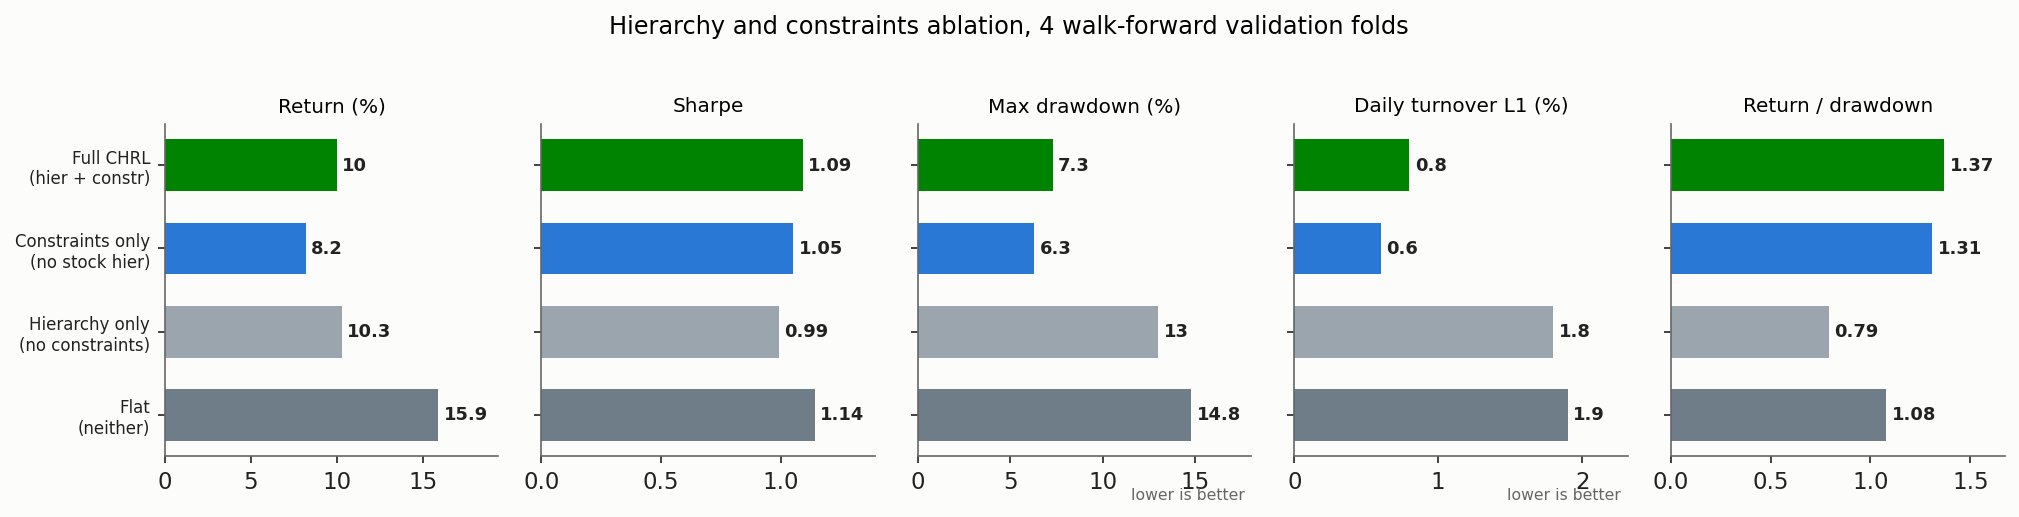
\includegraphics[width=\linewidth]{figures/fig_chrl_ablation.png}
  \caption{Rebuilding generation 1 four ways, each tested on 4 walk-forward folds. Bars show,
  left to right per panel: the full agent; rails without staged structure; structure without
  rails; neither. Panels, left to right: annual return (\%); Sharpe ratio; maximum drawdown (\%); daily
  trading volume (\% of the book turned over); and return/drawdown --- annual return divided
  by the worst peak-to-trough loss, the risk-adjusted summary. The rails halve the worst loss
  and the trading volume; structure alone is the worst variant; only the combination gets the
  best ratio.}
  \label{fig:ablation}
\end{figure}

\textbf{Generation 2 --- the best after-the-fact reading of that black box.} With the trained
agent frozen, we logged its internal states, clustered them into eight recurring
``behavior patterns'', labeled each from the trading record, and then \emph{intervened}:
nudged the internal state toward or away from a chosen pattern and passed the edited state
through the unchanged action network, so any behavioral change is attributable to the nudge.
The central methodological lesson: a nudge toward a \emph{random} target also ``improves'' results ($+0.55$ percentage points
of cumulative return over the frozen 2022--23 test window) --- gentle noise
shakes a slightly suboptimal policy off its habits --- so every claimed effect is reported
\emph{minus} its random-nudge control. Under that discipline, targeted edits genuinely work
($+0.19$ to $+0.30$ percentage points, control-adjusted). And the same program measures where
after-the-fact reading stops: a story limited to nine rules reproduces only $24.4\%$ of the
deployed agent's decisions; there is no way to bound what else an internal edit touches; and
the ${\sim}214$ knobs contain no command a human could name (Figure~\ref{fig:interp}).

\begin{figure}[h]
  \centering
  \includegraphics[width=\linewidth]{figures/fig_interp.png}
  \caption{The after-the-fact program. Left: its pipeline over the frozen agent --- log
  internal states, discover eight recurring behavior patterns, label them, intervene, and
  control every claim against random-target nudges. Right: the flagship effects, raw and
  after subtracting the random-nudge control (the dotted line is the random nudge itself ---
  the reason controls are mandatory).}
  \label{fig:interp}
\end{figure}

\textbf{Generation 3 --- the agent rebuilt readable (CRYSTAL-1).} Each measured wall becomes
an architectural decision. The agent's \emph{entire} memory is one named number: the
probability $b_t$ that the market is in a falling (``bear'') regime, updated daily by an
explicit two-regime Bayesian filter,
\begin{equation}
b_t \;=\; \frac{f_{\text{bear}}(r_t)\,\tilde b_t}
{f_{\text{bear}}(r_t)\,\tilde b_t + f_{\text{bull}}(r_t)\,(1-\tilde b_t)},
\qquad
\tilde b_t = \pi_{BB}\, b_{t-1} + \pi_{GB}\,(1-b_{t-1}),
\label{eq:belief}
\end{equation}
where $r_t$ is the day's market return, $f_{\text{bear}}$ and $f_{\text{bull}}$ are the
statistical profiles of daily returns in falling and rising regimes, $\tilde b_t$ carries
yesterday's belief forward through the regimes' persistence probabilities
($\pi_{BB}$: bear stays bear; $\pi_{GB}$: bull turns bear --- $B$ for bear, $G$ for the
good regime), and the ratio is Bayes' rule.
Because $b_t$ is the \emph{only} memory, the effect of writing to it is bounded by
construction --- the guarantee generation 2 could test for but never provide. The policy is a
small decision tree over $[b_t,\ \text{holdings},\ \text{time}]$ at full performance parity
(the readable form gives up none of the unconstrained version's performance); in its
certified form --- ``certified'' meaning it passed the frozen statistical exam of the
companion paper, including placebo controls, before its one pre-registered test --- it
degenerates to one sentence: \emph{if $b_t > 0.66$, cut stock exposure to $74\%$}.

\section{The measurement: a score that can lose}
\label{sec:metrics}

\begin{equation}
\textsc{CrystalScore} \;=\; F \times S \times S\!t,
\label{eq:cs}
\end{equation}
computed identically for every agent, where each factor is between 0 and 1:
\begin{itemize}
  \item $F$ (\textbf{faithfulness}): the fraction of \emph{command tests} that succeed --- set
        the belief to a chosen value and check the action changes exactly as the name
        promises, judged against what an ideal holder of that belief would do (the optimal
        action given that belief under the world model that defines the regimes). This is a
        causal test, per the standard of \S\ref{sec:ask}(2), not a visual inspection.
  \item $S$ (\textbf{simulatability}): the fraction of the agent's decisions reproduced by a
        story of at most nine named rules, under the constraint that the story-following agent \emph{performs as well as the
        original} --- a story that only explains a crippled version of the agent is
        cheating. Nine rules is a working-memory-sized budget; the measure is a
        program-executable proxy for human simulatability.
  \item $S\!t$ (\textbf{stability}): the fraction of independent retrainings (different
        random seeds) in which the same mechanism reappears.
\end{itemize}
One calibration lesson is itself a result. In a synthetic environment where the optimal
rule is known, we trained an agent to follow that rule ($97\%$ action agreement) --- an agent
that \emph{is} the rule for all practical purposes. Our first faithfulness test still
returned $F=0$ on it, because the test's fixed-size belief nudges never crossed the rule's
decision threshold. The repaired test writes contrasting values on both sides of the
threshold; under it, taught agents in the calibration environment read $F=0.77$--$0.83$ and
untaught ones still read $0$, while the deployed agents of Table~\ref{tab:glance} read
$F=1.0$. \emph{Interpretability metrics are instruments, and instruments need calibration.}

\section{Results}
\label{sec:results}

\begin{table}[h]
\centering\footnotesize
\begin{tabular}{p{3.7cm}p{6.4cm}p{4.0cm}}
\toprule
result & what was measured & evidence / protocol \\
\midrule
one score, three generations & black box $+$ its reading: $F{=}1.00 \times S{=}0.244
\times S\!t{=}0.619 = \mathbf{0.151}$; rebuilt readable: $F{=}1.00 \times S{=}0.92 \times
S\!t{=}1.00 = \mathbf{0.92}$ (for the black box, stability $=$ the share of retrainings in
which the same discovered mechanism recurs) & identical protocol, real market data, nine-rule
story budget \\[3pt]
the discriminating axis & command tests succeed on \emph{both} ($F=1.0$) --- command success cannot tell the designs apart; the story axis can: $24.4\%$ vs $92\%$ of decisions reproduced at equal performance & the paper's central finding \\[3pt]
a writable belief & writing the belief moves behavior exactly as named in $100\%$ of contrast tests; the state named ``bear'' is verifiably the state where de-risking is optimal; the mechanism reappears in $10/10$ retrainings; a proposed belief boost failed the pre-set non-inferiority threshold --- no edit may degrade
the certified objective --- and was correctly \emph{refused} & causal command tests, not visual inspection \\[3pt]
the certified sentence & ``if $b_t>0.66$, cut stock exposure to $74\%$'' beat buy-and-hold on the pre-registered
primary endpoint --- risk-adjusted improvement vs a matched twin, observed $z=2.06$
(${\sim}95\%$ confidence) --- with Sharpe $1.46$ vs $1.39$ and a smaller worst loss
($-12.9\%$ vs $-15.5\%$) & one pre-registered test on 629 unseen trading days \\[3pt]
after-the-fact reading: real but bounded & targeted internal edits help by $+0.19$--$0.30$ percentage points \emph{after} subtracting the random-nudge control ($+0.55$\,pp raw --- controls are mandatory); the nine-rule story ceiling is $24.4\%$ & frozen agent, matched-random controls \\[3pt]
where the risk result comes from & return/drawdown: full agent $1.37$; rails only $1.31$; structure only $0.79$; neither $1.08$ & 4-way rebuild, 4 walk-forward folds \\[3pt]
metric calibration & the strict command test read $F=0$ on an agent that \emph{is} the rule ($97\%$ clone); the repaired test reads $0.77$--$0.83$ on taught agents and still $0$ on untaught ones & a designed environment with known ground truth \\
\bottomrule
\end{tabular}
\caption{Results at a glance. Sharpe ratio $=$ annualized return divided by its volatility
(risk-adjusted return); worst loss $=$ maximum peak-to-trough decline; pp $=$ percentage
points; walk-forward $=$ train on one period, test on the next, roll forward.}
\label{tab:glance}
\end{table}

Beyond the table, one comparison summarizes the paper (Figure~\ref{fig:score}): the two
architectures scored on the same three axes. Command success ($F$) is $1.0$ for both --- a
black box can be steered too, which is why steering demonstrations, the most common evidence
in this literature, do not establish interpretability. What separates the designs is whether
a human-sized story can \emph{be} the agent: $24.4\%$ versus $92\%$ of decisions reproduced
at equal performance. Building the concepts in --- rather than discovering them afterwards ---
is worth a factor of ${\sim}4$ on the story axis and a factor of $6$ on the combined score,
at zero cost in trading performance.

\begin{figure}[h]
  \centering
  \includegraphics[width=.88\linewidth]{figures/fig_crystalscore.png}
  \caption{The same score on both architectures, real data only. Left group of bars:
  faithfulness (command tests), identical for both. Middle: simulatability (the nine-rule
  story), the discriminating axis. Right: stability across retrainings, and the combined
  \textsc{CrystalScore}.}
  \label{fig:score}
\end{figure}

\section{The claim, and the request}
\label{sec:claim}

The paper will claim: \textbf{(i)} the first quantitative comparison of a black box, its best
after-the-fact explanation program, and a rebuilt-readable successor under one metric that can
lose, on a real high-stakes task --- the evaluation instrument the surveys of
\S\ref{sec:ask} explicitly request; \textbf{(ii)} the finding that command success does not
discriminate architectures while parity-constrained simulatability does; \textbf{(iii)} the
first deployed agent whose belief state is a named, writable, certified interface ---
including the safety bar that refused an unsafe write; \textbf{(iv)} the calibration lesson
that interpretability metrics are instruments requiring ground-truth surfaces. A companion
paper (\emph{Hello Crystal}) covers the statistically governed self-improvement loop that
modifies this agent; its safety precondition --- \emph{an agent may change itself only to the
degree it can be read} --- is exactly what this paper makes measurable. All results are
complete, logged, and audited; this document requests approval to write the full paper.

\bibliographystyle{plainnat}
\bibliography{refs}

\end{document}
